\documentclass{article}

\usepackage[utf8]{inputenc}
\usepackage[portuguese]{babel}
\usepackage{blindtext}
\usepackage{graphicx}
\usepackage{amsmath}
\usepackage{float}
\usepackage{caption}
\usepackage[compact]{titlesec}
\usepackage{multicol}
\usepackage[a4paper, total={7.5in, 10in}]{geometry}
\usepackage[font=scriptsize,labelfont=bf]{caption}
\usepackage{listings}
\usepackage{color}
 
\definecolor{codegreen}{rgb}{0,0.6,0}
\definecolor{codegray}{rgb}{0.5,0.5,0.5}
\definecolor{codepurple}{rgb}{0.58,0,0.82}
\definecolor{backcolour}{rgb}{0.95,0.95,0.92}
 
\lstdefinestyle{mystyle}{
    backgroundcolor=\color{backcolour},   
    commentstyle=\color{codegreen},
    keywordstyle=\color{magenta},
    numberstyle=\tiny\color{codegray},
    stringstyle=\color{codepurple},
    basicstyle=\footnotesize,
    breakatwhitespace=false,         
    breaklines=true,                 
    captionpos=b,                    
    keepspaces=true,                 
    numbers=left,                    
    numbersep=5pt,                  
    showspaces=false,                
    showstringspaces=false,
    showtabs=false,                  
    tabsize=2
}
 
\lstset{style=mystyle}

\setlength{\columnsep}{1cm}
\setlength{\parindent}{0em}
\titlespacing{\section}{1pt}{*-0.55}{*-0.8}
\begin{document}

\textbf{Relatório de Entrega de Trabalho} \newline
\textbf{Disciplina de Programação Paralela (PP)}\textbf{ - Prof. César De Rose} \newline
\textbf{Alunos:} Rafael Rios e Rodrigo Silveira \newline
\textbf{Exercício:} TPP3: MPI Fases Paralelas (FP)

\begin{multicols*}{2}

\section{Implementação}
O objetivo deste trabalho foi implementar usando a biblioteca MPI um algoritmo seguindo o modelo de fases paralelas para ordenar um vetor de 1000000 de elementos usando bubblesort. Cada processo recebe uma parte igual do vetor e a ordena localmente, verificando se o mesmo está ordenado em relação aos processos vizinhos e, se não está, realiza-se trocas de seus elementos visando a ordenação completa do vetor. Os processos seguem a ordem de seus respectivos índices, em uma lista da esquerda para a direita de 0 até np-1, a implementação se inicia com cada vetor local sendo criado dentro do seu respectivo processo e recebendo 1/(np-1) avos do tamanho total, o vetor é inicializado em ordem decrescente (pior caso) e um vetor auxiliar (vet\_pronto) é criado para armazenar o estado de todos os processos, cada posição corresponde ao seu índice, com valores '1' se o vetor local daquele processo está ordenado, e '0' quando não está. Os vetores são ordenados usando bubblesort e compara-se o maior valor do vetor, com o menor valor do vetor do processo a sua direita (para todos, menos para o processo 0, que só envia o elemento), se o dado enviado for menor, o vetor está ordenado em relação ao seu vizinho, atualizando o vet\_pronto com seu respectivo índice para '1'. Através da função MPI\_Bcast, é feita a atualização dos vet\_pronto de todos os processos, conferindo se é o fim da execução (todas as posições em '1'). A troca de elementos é realizada através de posições auxiliares nos vetores locais, fixou-se o tamanho do número de elementos da troca em 1,5\% do total (1000000), cada processo (exceto o 0) envia essa quantidade de seus menores valores para o vizinho à esquerda, o qual recebe e ordena esses elementos com a mesma quantidade de seus maiores valores, devolvendo para o processo que enviou os maiores elementos após essa ordenação. O algoritmo retorna para a etapa de ordenação do vetor completo, percorrendo novamente o algoritmo, todos os processos executam o mesmo código, até haver a ordem completa dos vetores.
\section{Dificuldades encontradas}
Uso correto da função MPI\_Bcast, de maneira a manter o sincronismo do vetor pronto; Desenvolvimento da inicialização dos vetores localmente, visto que, no inicio, tentou-se criar um único vetor total e dividi-lo entre os processos, não obtendo sucesso; Escolha da melhor quantidade de elementos a serem trocados entre os vetores de modo a convergir de maneira mais rápida para a solução desejada.  
\section{Testes}
Foram realizados testes com alocação de 2 nodos na grad, executando o código para 16 e 32 processos, em ambos os casos, testou-se para diferentes quantidades de elementos sendo trocados entre os processos, visando obter o melhor resultado possível. A primeira execução foi realizada com 0.25\% do tamanho total do vetor (1000000), a cada novo teste, aumentou-se esse valor em 0.25\%, percebendo que após 1.5\% o tempo de execução não aumentava, e para valores muito maiores, o algoritmo sequer convergia para a solução requisitada, ao final dos testes, o melhor resultado obtido foi 553.4 segundos para 16 processos e 358.3 segundos para 32 (HT).
\section{Análise de desempenho}
A versão paralela do algoritmo melhorou o resultado em comparação com a execução sequencial, obtendo menores tempos de execução, todavia a eficiência ficou abaixo do ideal, para ambos os números de processos, atingindo 0.5 de eficiência (D) para 16 processos e 0.4 para 32 (E). O speed-up obtido também foi abaixo do ideal, 8 para 16 processos e 12.4 para 32. Em comparação com o algoritmo de divisão e conquista (D\&C) do trabalho anterior, o resultado do fases paralelas foi muito inferior, como pode ser visto na Figura 1, as barras A, B e C correspondem a eficiência das três execuções do algoritmo divisão e conquista, código até o HT, ordenamento local e código padrão após o HT, respectivamente, demonstrando a grande diferença de performance em comparação a ordenação do fases paralelas, isto ocorre pois o algoritmo desse trabalho não é projetado para solucionar esse tipo de problema, gastando muito mais tempo ordenando do que realizando a comunicação, demorando para convergir.  
\begin{figure}[H]
            \centering
            \vspace{-1.1em}
            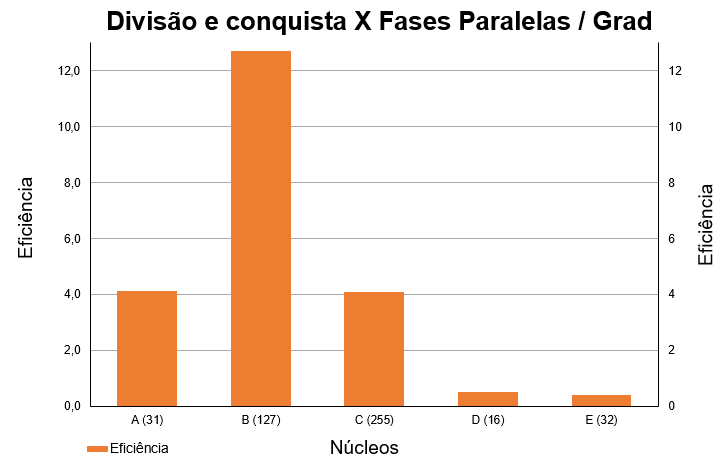
\includegraphics[width=9cm, height=5cm]{Capture.PNG}
            \vspace{-1.9em}
            \caption{Gráfico de eficiência comparando D\&C(A,B,C) com FP(D,E)}
            \vspace{-1.2em}
\end{figure}
\section{Observações Finais}
A utilização do algoritmo de fases paralelas se mostrou mais eficiente que a execução sequencial, como era esperado, porém, não foi o melhor algoritmo visto no decorrer da disciplina, ficando atrás dos outros dois processamentos paralelos abordados em aula, o mestre-escravo e o divisão e conquista. Obteve-se resultados razoáveis de speed-up e eficiência, entretanto também foram inferiores aos valores obtidos na execução dos outros algoritmos vistos. É importante analisar a diferença nos tempos medidos para as alterações da quantidade de elementos trocados entre os vetores para realizar a ordenação de maneira correta, sendo este o aspecto mais intrínseco do algoritmo.

\end{multicols*}

\newpage

\lstinputlisting[language=C++]{tpp3.c}

\end{document}
